\chapter{Analisis}
\label{chap:analisis}
Bab ini berisi analisis masalah dan solusi, studi kasus, perancangan perangkat lunak, diagram aktivitas, \textit{use case} diagram, dan diagram paket.


\section{Analisis 3 Dimensi}
\label{sec:3dimensi}

Pada dunia 3 dimensi terdapat berbagai jenis penerangan, pemodelan, dan juga bentuk-bentuk yang mendukung untuk implementasi pembuatan ruang kelas pada Fakultas Teknologi Informasi dan Sains secara 3 dimensi. Penerangan, pemodelan, dan bentuk-bentuk yang digunakan pada dunia 3 dimensi akan dijelaskan pada subbab di bawah ini.

\subsection{Analisis Penerangan 3 Dimensi}
\label{sec:lighting}
Pada dunia 3 dimensi dan khususnya pada pemanfaatan pustaka Three.js, telah disediakan berbagai macam penerangan untuk memberikan pencahayaan pada layar. Contoh penerangan yang disediakan oleh pustaka Three.js adalah {\it AmbientLight, DirectionalLight, Hemisphere Light, PointLight, RectAreaLight} dan {\it SpotLight}. Namun pada implementasi kelas Fakultas Teknologi Informasi dan Sains ke dalam model 3 dimensi tidak digunakan penerangan, hal tersebut terjadi karena telah digunakan material yang dapat terlihat meskipun tanpa ada cahaya pada layar tersebut. Material tersebut adalah {\it MeshBasicMaterial}, sebuah material yang paling sederhana dan tidak memperhitungan cahaya.

\subsection{Analisis Pemodelan Properti Kelas}
\label{sec:pemodelanproperti}
Pemodelan properti kelas merupakan proses dibuatnya masing-masing satuan properti yang dimiliki oleh kelas pada Fakultas Teknologi Informasi dan Sains. Pada proses pemodelan akan dilakukan pembentukan properti kelas pada editor hingga menyerupai bentuk asli dari properti yang sedang dimodelkan. Penulis memanfaatkan bantuan aplikasi Blender dalam melakukan pemodelan properti kelas. Aplikasi Blender merupakan sebuah perangkat lunak untuk membangun grafika 3 dimensi. Terdapat 2 buah tahapan dalam memodelkan suatu bentuk properti, yaitu sebagai berikut:
\begin{itemize}
	\item {\bf Pembentukan model}, pada tahap ini dilakukan berbagai cara untuk memanipulasi bentuk model hingga bentuknya menyerupai properti yang asli. Dilakukan berbagai usaha untuk dapat menyerupai bentuk dari properti asli seperti {\it selecting, extruding, rotating, scaling, moving}, dan lain-lain. Pada gambar ~\ref{fig:modelling1} dapat dilihat proses pembentukan model untuk properti meja dosen.
	\item {\bf Pemetaan tekstur}, pada tahap ini dilakukan pemetaan permukaan objek ke gambar tekstur yang cocok dengan model tersebut. Setiap bagian permukaan dari model akan dibuka hingga menjadi satu permukaan datar. Kemudian permukaan datar tersebut akan ditempelkan kepada tekstur yang cocok dengan model tersebut. Pada gambar ~\ref{fig:uvwrap1} dapat dilihat proses pembukaan setiap permukaan dari model meja dosen hingga menjadi satu permukaan datar. Lalu kemudian hasil akhirnya dapat dilihat pada gambar ~\ref{fig:modelwarna1}.
	\begin{figure}
		\centering
		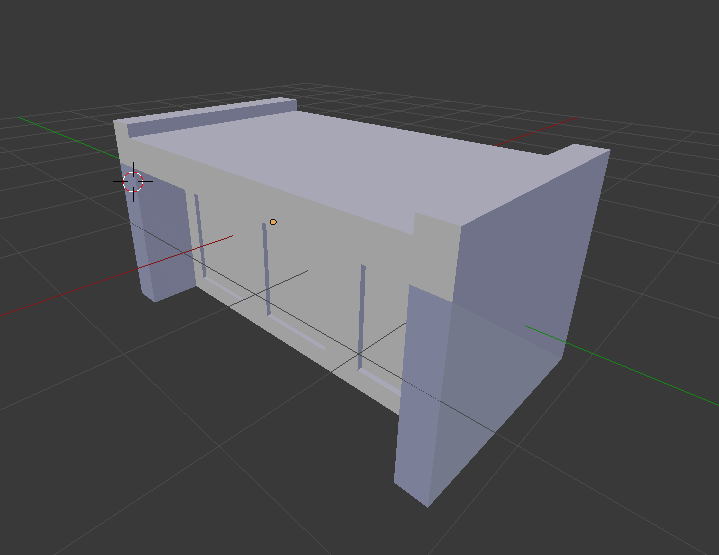
\includegraphics[scale=0.5]{modelling1}
		\caption{Pembentukan model properti meja dosen}
		\label{fig:modelling1}
	\end{figure}
	\begin{figure}
		\centering
		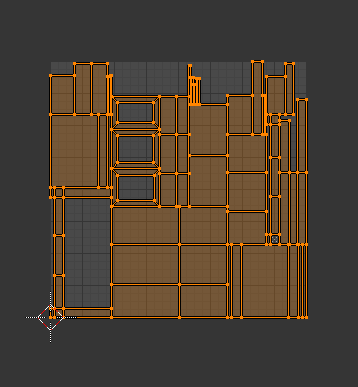
\includegraphics[scale=0.8]{uvwrap1}
		\caption{Pembukaan setiap bagian permukaan dari model meja dosen hingga menjadi satu permukaan datar}
		\label{fig:uvwrap1}
	\end{figure}
	\begin{figure}
		\centering
		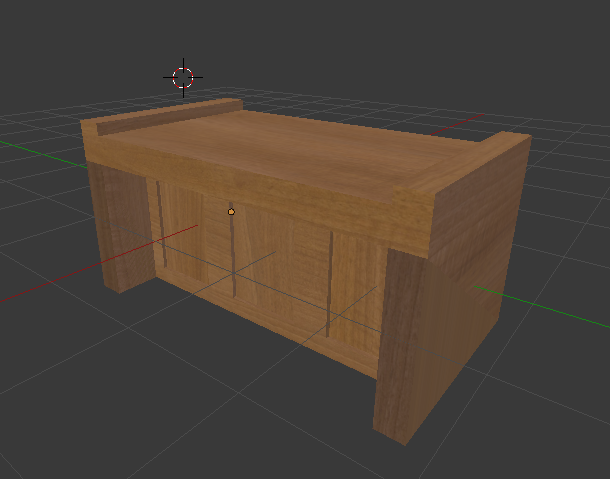
\includegraphics[scale=0.6]{modelwarna1}
		\caption{Hasil akhir pemodelan properti meja dosen}
		\label{fig:modelwarna1}
	\end{figure}
\end{itemize}

\subsection{Pemanfaatan pustaka Three.js pada implementasi pemodelan Aplikasi Pratinjau 3 Dimensi Berbasis Web}
\label{sec:pemanfaatanthreejs}
Pada pengimplementasian Aplikasi Pratinjau 3 Dimensi Berbasis Web digunakan banyak fitur yang telah disediakan oleh pustaka Three.js. Berikut ini merupakan daftar fitur pustaka Three.js yang digunakan pada implementasi Aplikasi Pratinjau 3 Dimensi Berbasis Web:
\begin{itemize}
	\item {\bf Scene}, merupakan sebuah layar atau wadah untuk menempatkan sesuatu pada pustaka Three.js. {\it Scene} harus selalu diimplementasikan karena merupakan elemen dasar yang diperlukan pada representasi grafika 3 dimensi. Contoh penggunaan {\it Scene} pada implementasi Aplikasi Pratinjau 3 Dimensi Berbasis Web dapat dilihat pada {\it listing} ~\ref{fig:scene}.
\begin{lstlisting}[caption={Contoh penggunaan {\it Scene} pada implementasi Aplikasi Pratinjau 3 Dimensi Berbasis Web dengan latar warna putih}, label={fig:scene},captionpos=b]
	var scene = new THREE.Scene();
	scene.background = new THREE.Color(constant.worldColor);
\end{lstlisting}
	\item Color
	\item {\bf PerspectiveCamera}, merupakan kamera yang menggunakan proyeksi perspektif. Terdapat juga jenis kamera lain seperti {\it CubeCamera} dan {\it OrthographicCamera}, namun pada implementasi Aplikasi Pratinjau 3 Dimensi Berbasis Web yang digunakan adalah {\it PerspectiveCamera} karena lebih cocok dalam representasi yang menyerupai perspektif dunia nyata. Contoh penggunaan {\it PerspectiveCamera} pada implementasi Aplikasi Pratinjau 3 Dimensi Berbasis Web dapat dilihat pada {\it listing} ~\ref{lst:perspectiveCam}.
\begin{lstlisting}[caption={Contoh penggunaan {\it PerspectiveCamera} pada implementasi Aplikasi Pratinjau 3 Dimensi Berbasis Web dengan pengaturan kamera dan posisi tertentu}, label={lst:perspectiveCam},captionpos=b]
	var camera = new THREE.PerspectiveCamera(75, window.innerWidth/
	window.innerHeight, 0.1, 100, 100);
    	camera.position.set(0, 10, 40);
\end{lstlisting}
	\item WebGLRenderer merupakan pembangun model 3 dimensi untuk ditampilkan ke layar. Fitur ini menyediakan tempat untuk membangun {\it Scene} dan berbagai hal 3 dimensi lainnya. Contoh penggunaan {\it WebGLRenderer} pada implementasi Aplikasi Pratinjau 3 Dimensi Berbasis Web dapat dilihat pada {\it listing} ~\ref{lst:webglRenderer}.
\begin{lstlisting}[caption={Contoh penggunaan {\it WebGLRenderer} pada implementasi Aplikasi Pratinjau 3 Dimensi Berbasis Web dengan batasan area hanya pada elemen {\it canvas}}, label={lst:webglRenderer},captionpos=b]
	    var renderer = new THREE.WebGLRenderer(
	    {canvas: document.getElementById('canvas'), antialias: true});
\end{lstlisting}
	\item OrbitControls 
	\item JSONLoader, merupakan pemuat objek dalam bentuk JSON (JavaScript Object Notation). Pemuat ini mengubah format JSON menjadi objek yang dapat dibaca oleh pustaka Three.js. Pada implementasi Aplikasi Pratinjau 3 Dimensi Berbasis Web, {\it JSONLoader} digunakan untuk membaca model properti kelas yang sebelumnya telah disimpan dalam format JSON. Contoh penggunaan {\it JSONLoader} pada implementasi aplikasi ini dapat dilihat pada {\it listing} ~\ref{lst:jsonLoader}.
\begin{lstlisting}[caption={Contoh penggunaan {\it JSONLoader} pada implementasi Aplikasi Pratinjau 3 Dimensi Berbasis Web}, label={lst:jsonLoader},captionpos=b]
	   var loader = new THREE.JSONLoader();
            var callbackProperty = function(geometry) {
                var texture = new THREE.TextureLoader().load(property.texture);
                var material = new THREE.MeshBasicMaterial( { map : texture } ); 
                var mesh = new THREE.Mesh(geometry, material);
                mesh.position.set(dx,dy,dz);
                mesh.scale.set(property.scale,property.scale,property.scale);
                mesh.rotation.y = property.rotation;
                scene.add(mesh);
            };
            loader.load(property.model, callbackProperty);
\end{lstlisting}
	\item TextureLoader, merupakan pemuat untuk gambar tekstur. Pada implementasi Aplikasi Pratinjau 3 Dimensi Berbasis Web, {\it TextureLoader} digunakan untuk memuat gambar tekstur yang kemudian akan digunakan untuk model properti kelas. Contoh penggunaan {\it TextureLoader} pada implementasi aplikasi ini ada pada {\it listing} ~\ref{lst:texLoader}.
\begin{lstlisting}[caption={Contoh penggunaan {\it TextureLoader} untuk tekstur suatu {\it mesh} yang akan ditambahkan ke {\it Scene} pada implementasi Aplikasi Pratinjau 3 Dimensi Berbasis Web}, label={lst:texLoader},captionpos=b]
  	var texture = new THREE.TextureLoader().load(property.texture);
         var material = new THREE.MeshBasicMaterial( { map : texture } ); 
         var mesh = new THREE.Mesh(geometry, material);
          mesh.position.set(dx,dy,dz);
          mesh.scale.set(property.scale,property.scale,property.scale);
          mesh.rotation.y = property.rotation;
          scene.add(mesh);
\end{lstlisting}
	\item MeshBasicMaterial, merupakan sebuah bahan untuk menggambar geometri dengan cara yang sederhana dan datar. Pada implementasi Aplikasi Pratinjau 3 Dimensi Berbasis Web, {\it MeshBasicMaterial} digunakan untuk semua geometri yang ada seperti properti kelas dan ruangan kelas itu sendiri. Contoh penggunaan {\it MeshBasicMaterial} dapat dilihat pada {\it listing} ~\ref{lst:meshBasicMat}.
\begin{lstlisting}[caption={Contoh penggunaan {\it MeshBasicMaterial} untuk suatu {\it mesh} yang akan ditambahkan ke {\it Scene} pada implementasi Aplikasi Pratinjau 3 Dimensi Berbasis Web}, label={lst:meshBasicMat},captionpos=b]
	var texture = new THREE.TextureLoader().load(property.texture);
	var material = new THREE.MeshBasicMaterial( { map : texture } ); 
	var mesh = new THREE.Mesh(geometry, material);
	mesh.position.set(dx,dy,dz);
	mesh.scale.set(property.scale,property.scale,property.scale);
	mesh.rotation.y = property.rotation;
	scene.add(mesh);
\end{lstlisting}
	\item Mesh, merupakan sebuah bentuk representasi objek. Pada implementasi Aplikasi Pratinjau 3 Dimensi Berbasis Web, {\it Mesh} digunakan untuk objek properti kelas. Contoh penggunaan {\it Mesh} dapat dilihat pada listing ~\ref{lst:mesh}
\begin{lstlisting}[caption={Contoh penggunaan {\it Mesh} yang akan ditambahkan ke {\it Scene} pada implementasi Aplikasi Pratinjau 3 Dimensi Berbasis Web}, label={lst:mesh},captionpos=b]
  	var texture = new THREE.TextureLoader().load(property.texture);
         var material = new THREE.MeshBasicMaterial( { map : texture } ); 
         var mesh = new THREE.Mesh(geometry, material);
          mesh.position.set(dx,dy,dz);
          mesh.scale.set(property.scale,property.scale,property.scale);
          mesh.rotation.y = property.rotation;
          scene.add(mesh);
\end{lstlisting}
	\item BoxGeometry, merupakan sebuah geometri berbentuk segi empat. Pada implementasi Aplikasi Pratinjau 3 Dimensi Berbasis Web {\it BoxGeometry} digunakan sebagai representasi dari ruangan kelas. Contoh penggunaan {\it BoxGeometry} dapat dilihat pada {\it listing} ~\ref{lst:boxGeo}.
\begin{lstlisting}[caption={Contoh penggunaan {\it BoxGeometry} sebagai kelas yang akan ditambahkan ke {\it Scene} pada implementasi Aplikasi Pratinjau 3 Dimensi Berbasis Web}, label={lst:boxGeo},captionpos=b]
  	var geometry = new THREE.BoxGeometry(length, width, height);
        var material = new THREE.MeshFaceMaterial(cubeMaterials);
        var cube = new THREE.Mesh(geometry, material);
        cube.position.y = 9.05;
        cube.name = 'room';
        scene.add(cube);
\end{lstlisting}
	\item MeshFaceMaterial, merupakan 
	\item Vector3
\end{itemize}

\section{Analisis Struktur Web}
\label{sec:analisisStrukturWeb}

Struktur web merupakan susunan direktori yang membangun web tersebut. Struktur web terdiri dari berbagai folder dan berkas yang telah dipisahkan berdasarkan fungsinya masing-masing. Berikut ini merupakan penjelasan masing-masing folder dan berkas yang digunakan untuk membangun web ini:

\begin{itemize}
	\item {\bf folder css}, folder ini berisi berkas dengan ekstensi css yang digunakan untuk mengatur dan memperindah tampilan web. Berkas yang ada pada folder ini hanya satu yaitu custom.css.
	\item {\bf folder img}, folder ini berisi berkas gambar dengan ekstensi jpg. Terdapat banyak berkas gambar seperti tekstur, pilihan warna cat dinding, pilihan warna lantai, dan gambar-gambar lainnya yang berkaitan dengan Aplikasi Pratinjau 3 Dimensi Berbasis Web.
	\item {\bf folder js}, folder ini berisi berkas dengan ekstensi js. Terdapat berbagai file JavaScript di dalam folder ini, contohnya adalah sebagai berikut:
		\begin{itemize}
			\item {\bf Main.js}, berkas JavaScript ini berisi berbagai fungsi utama yang digunakan untuk membangun Aplikasi Pratinjau 3 Dimensi Berbasis Web.
			\item {\bf three.js}, berkas JavaScript ini berisi berbagai fungsi yang disediakan oleh pustaka Three.js. Nantinya fungsi yang terdapat di dalam berkas ini akan dipanggil oleh Main.js
			\item {\bf OrbitControls.js}, berkas JavaScript ini berisi berbagai fungsi yang juga disediakan oleh pustaka Three.js. Namun pada berkas ini hanya khusus menyediakan fungsi-fungsi yang berkaitan dengan kontrol pada kamera.
		\end{itemize}
	\item {\bf folder json}, folder ini berisi berkas dengan ekstensi JSON. Terdapat 2 berkas json di dalam folder ini yaitu sebagai berikut:
		\begin{itemize}
			\item {\bf constant.json}, berkas ini berisi berbagai informasi awal untuk diinisialisasi ke aplikasi sehingga dapat menampilkan gambaran awal dari ruangan kelas Fakultas Teknologi Informasi dan Sains.
			\item {\bf imported.json}, berkas ini berisi informasi untuk repsentasi ruangan kelas saat ujian sedang berlangsung di Fakultas Teknologi Informasi dan Sains.
		\end{itemize}
	\item {\bf folder models}
	\item {\bf berkas index.html}
\end{itemize}












